\documentclass{article}  % list options between brackets
\usepackage{bmpsize}
\usepackage[dvipdfmx]{graphicx}              % list packages between braces
\usepackage{url}
\usepackage{color}
\usepackage{amsmath}
\usepackage{amsfonts}
\usepackage{hyperref}

% type user-defined commands here

\begin{document}

\title{Expectation Maximization}   % type title beTrending Predictiontween braces
\author{greeness}         % type author(s) between braces
\maketitle


\section{Introduction}

The EM algorithm is an efficient iterative procedure to compute the Maximum Likelihood (ML) estimate in the presence of missing or hidden data~\cite{sb}. In ML estimation, we wish to estimate the model parameter(s) for which the observed data are the most likely.

Each iteration of the EM algorithm consists of two processes. The E-step and the M-step. In the expectation, or E-step, the missing data are estimated given the observed data and the current estimate of the model parameters. This is achieved using the conditional expectation, explaining the choice of terminology. In the M-step, the likelihood function is maximized under the assumption that the missing data are known The estimate of the missing data from the E-step are used in lieu of the actual missing data~\cite{sb}.

There are two main applications of the EM algorithm. 
\begin{itemize}
  \item When the data indeed has missing values, due to limitations of the
  observation proess.
  \item When optimizing the likelihood function is analytically intractable.
  However, by assuming the existence of certain hidden or latent variables, the
  probelm could be simplified and easier to handle. s
\end{itemize}
\section{Notations} 
Here we list the notations used:
\begin{enumerate}
  \item math functions
  \begin{itemize}
    \item $p(.)$ or $P(.)$, probability density function (pdf) or probability
    mass function;
    \item $E[.]$, expectation;
    \item $\frac{\partial f}{\partial x}$, partial derivative w.r.t $x$;
    \item $C_m^k$, $m$ choose $k$ or the binomial coefficients.
  \end{itemize}
  \item case: complete data
  \begin{itemize}
  \item $Y$, the randoam variable that we can observe its realizations;
  \item $y$, observed data or data vector (constant, instantiation or
  realization of the random variable $Y$);
  \item $\theta$, parameters for the statistical representation of the data model;
  \item $\theta_n$, the estimate of $\theta$ at the $n$th iteration (constant);
  \item $l(\theta)=P(y|\theta)$, likelihood function, i.e., how likely the
  observed data are generated by the parameters;
  \item $L(\theta) = \log P(y|\theta)$, log-likelihood function, or denoted as
  $L$;
  \item $J$, total number of observations. $y_j$, the $j$th observation;
  \end{itemize}
  \item case: incomplete data (additional notations)
  \begin{itemize}
  \item $Z$, hidden random variable
  \item $z$, unobserved/missing data (instantiation of the hidden
  variable);
  \item $x$, complete data consisting of $(y,z)$, if there is no hidden
  variable, then $x\doteq  y$;  
  \item $X$: the underlying random varialble of $x$;
  \item $l(\theta)=P(x|\theta)=P(y,z|\theta)$, likelihood function for the
  complete data when we have hidden variable $z$;
  \item $L(\theta) = \log P(x|\theta)$, log-likelihood function for the
  complete data when we have hidden varialble $Z$, or denoted as $L$;
  \item $P(Z=z|y,\theta)$ or $P(z|y,\theta)$, given current parameters $
  \theta$ and the observed data $y$, what is the probability that the data is coming from $z$.
  \item $Q = Q(\theta|\theta_n)= E_{z|y,\theta_n}[\log P(x|\theta)]$, or
  $E_{z}[\log P(x|\theta) | y,\theta_n] $, or just $E[\log
  P(x|\theta)]$, the expected quantity we compute in
  E-step. The conditional expectation is with respective to $z$.
  \item $I$, total number of components in the mixture;  
  \end{itemize}
\end{enumerate}



\section{Short Review: Maximimum Likelihood}
The goal of Maximum Likelihood (ML) estimation is to find parameters that
maximize the probability of having received certain measurements(observations)
of a random variable distributed by some probability function (p.d.f)~\cite{em_mb}. For
example, we look at a random variable $Y$ and a measurement vector $y =
(y_1,\cdots,y_J)$. The probability of receiving some measurement $y_j$ is given
by the p.d.f:

\[
p(y_j|\theta),
\]

where the p.d.f. is governed by the parameter $\theta$. The probablility of
having received the whole series of measurements is then 
\[
p(y|\theta)=\prod _{j=1}^J p(y_j|\theta)
\]
if the measurements are independent. The likelihood function is defined as a
function of $\theta$:
\begin{equation}
l(\theta) = p(y|\theta).
\end{equation}
The ML estimate of $\theta$ is found by maximizing $l$. Often, it is easier to
maximize the log-likelihood:
\begin{align*}
L=\log l(\theta) = & \log p(y|\theta)\\
= & \log \prod_{j=1}^J p(y_j|\theta) \\
= & \sum _{j=1}^J \log p(y_j|\theta)
\end{align*}

Since the logarithm is a strictly increasing function, the maximum of $l$ and
$\log(l)$ is the same. 

\section{Coin Toss Example}

\subsection{Complete Data} A person has one biased coin. The probability of
the coin's landing at heads is $\theta$. The tossing scenario is as below: 
\begin{itemize}
\item Toss  the coin six times;
\item Observing data $y$: HHHTHT;
\end{itemize}
Suppose we want to know the ML estimate of the coin bias $\theta$:
Assume that you toss a $(\theta, 1-\theta)$ coin $m$ times and get $k$ heads and $m-k$ tails. 
The probability of getting $k$ heads and $m-k$ tails is
\[
P(y|\theta)=P(y_1,\cdots,y_m|\theta) = C_m^k \theta^k (1-\theta)^{m-k}
\]
following the pdf of binomial distribution. 
The log-likelihood of the data is:
\[
L(\theta)=\log P(y|\theta) = \log C_m^k\theta^k(1-\theta)^{m-k}
=\texttt{constant}+ k\log \theta + (m-k) \log (1-\theta).
\]


To maximize, set the derivative with respective to $\theta$ equal to zero:
\[
\frac{dL}{d\theta} = \frac {k}{\theta} - \frac{m-k}{1-\theta} = 0
\]
Solving this for $\theta$, gives $\tilde \theta = \frac{k}{m}$. 

% To know which coin is more likely to produce this sequence, we compute
% \begin{align*}
% &P(x \texttt{ was obtained from coin i})=\\
% &P(\texttt{coin i}|y) = \frac{P(y|\texttt{coin i})P(\texttt{coin i})}{P(y)} \\
% &= \frac{P(y|\theta_i)P(\texttt{coin i})}{P(y)} \\
% &\propto P(y|\theta_i)
% \end{align*}
% The posterior is proportional to the likelihood  because we assume each coin has equal priors:
% \[
% P(\texttt{coin 0}) = P(\texttt{coin 1}) = P(\texttt{coin 2})
% \]
% 
% Thus we just need to pick the coin with the maximum $ P(y|\texttt{coin i})$. 

\subsection{Incomplete Data} A person has three biased coins. The probability of
coin's landing at heads is $\lambda,p,q$ respectively. The tossing scenario is
as below:
\begin{itemize}
\item Toss coin 0;
\item If head, we toss coin 1 another 4 times;
\item Otherwise, we toss coin 2 another 4 times;
\item We can only observe the sequence produced by coins 1 and/or coin 2, which
are data $y_j, j \in 1,2,3,4$: HHHT, HTHT, HHHT, HTTH;
\item The goal is to estimate most likely values for $\theta = (\lambda, p,
q)^T$.
\end{itemize}

Thus we have no idea which of the data points came from coin 1 and which from coin 2. 
\begin{itemize}
\item Suppose $\theta_n = (\lambda_n, p_n, q_n)^T$ is the current estimate of
parameters, for simplicity, we just write as $(\lambda, p, q)^T$
\item Let $z$ be the hidden \emph{indicator} variable, which coin was tossed at the beginning of each attempt. If $z=1$, coin 1 was tossed; otherwise, coin 2 was tossed. 
\item What is the probability $P(z)$ given $\theta = (\lambda, p, q)^T$ and $y$?
Suppose there were $m$ coin tosses and $h_j$ heads in the $j$th coin toss $y_j$. 
\begin{align*}
P_j &= P(z_j=1|y_j,\theta)= P(\texttt{coin 1}|y_j,\theta) =
\frac{P(y_j|\texttt{coin 1}) P(\texttt{coin 1})}{P(y_j)}\\
P(\texttt {coin 1}) &= \lambda\\
P(\texttt {coin 2}) &= 1-\lambda\\
P(y_j|\texttt{coin 1}) &= p ^ {h_j} (1-p)^{m-h_j}\\
P(y_j|\texttt{coin 2}) &= q ^ {h_j} (1-q)^{m-h_j}\\
p(y_j) &= P(y_j|\texttt{coin 1}) p(\texttt{coin 1}) + P(y_j|\texttt{coin 2})
p(\texttt{coin 2})\\
            &=   p ^ {h_j} (1- p)^{m-h_j}  \lambda + q ^ {h_j} (1- q)^{m-h_j}
            (1- \lambda)
\end{align*}
Plug in all factors, we have,
\begin{align*}
P_j &= \frac{ p ^ {h_j} (1- p)^{m-h_j}  \lambda}{ p ^ {h_j} (1- p)^{m-h_j} 
\lambda +  q ^ {h_j} (1- q)^{m-h_j} (1-\lambda)}
\end{align*}

\item Considering $E(Z) = \sum_{z_j} z_j P(Z=z_j)$

The expectation of $z_j$ is: 
\begin{align*}
E[z_j] &= 1 \times P(y_j \texttt{ was obtained from coin 1}) + 0 \times P(y_j
\texttt{ was obtained from coin 2})\\
&= 1 \times P(z_j=1) + 0 \times P(z_j=0)\\
&= 1 \times P(z_j=1|y_j,\theta) + 0 \times P(z_j=0|y_j,\theta)\\
&= P_j.
\end{align*}


\item We want to maximize the log-likelihood of the data: $L=\log
P(y,z|\lambda,p,q)$. However, $z$ is hidden. We think of $L$ as a random variable that depends on $z$. Therefore, instead of maximizing the $L$, we maximize the expectation of this random variable.
\begin{align*}
P(y_j,1|\theta) &= \lambda p^{h_j}(1-p)^{m-h_j}\\
P(y_j,0|\theta) &= (1-\lambda) q^{h_j}(1-q)^{m-h_j}\\
P(y_j,z_j|\theta) &= \left( \lambda p^{h_j}(1-p)^{m-h_j}\right)^{z_j}
\left((1-\lambda) q^{h_j}(1-q)^{m-h_j}\right)^{1-z_j}\\
                                         &= \lambda ^{z_j} p^{z_jh_j}(1-p)^{z_j(m-h_j)} (1-\lambda)^{1-z_j}q^{(1-z_j)h_j}(1-q)^{(1-z_j)(m-h_j)}\\
\log P(y_j,z_j|\theta) &= z_j\log\lambda + z_jh_j\log p + z_j(m-h_j)\log (1-p) +
\\
& (1-z_j)\log (1-\lambda) + (1-z_j)h_j\log q + (1-z_j)(m-h_j)\log(1-q)
\end{align*} 

Combining all test trials, we have:
\begin{align*}
P(y,z|\theta) &= \prod _j P(y_j,z_j|\theta)\\
\log P(y,z|\theta) &= \log \prod _j P(y_j,z_j|\theta)\\
 &= \sum _j \log P(y_j, z_j|\theta)
\end{align*}

Considering $E(X+Y) = E(X) + E(Y)$, we get:

\begin{align*}
E\left[\log P(y,z|\theta) \right]&= E\left[\sum_j \log P(y_j,
z_j|\theta)\right]\\
&= \sum_j E\left[\log P(y_j, z_j|\theta)\right]
\end{align*}
Plug in $\log P(y_j, z_j|\theta)$, we get:

\begin{align*}
E\left[\log P(y,z|\theta) \right]&= \sum_j E [z_j\log\lambda + z_jh_j\log p +
z_j(m-h_j)\log (1-p) + \\
& (1-z_j)\log (1-\lambda) + (1-z_j)h_j\log q + (1-z_j)(m-h_j)\log(1-q)]
\end{align*}

Still remember $E[z_j] = P_j$? Also considering $E[kX] = kE[x], E[k+X] = k +
E[X]$, where $k$ is a constant.

\begin{align*}
Q= &E\left[\log P(y,z|\theta) \right]\\
= &\sum_j E[z_j]\log\lambda + E[z_j]h_j\log p + E[z_j](m-h_j)\log (1-p) + \\
& E[1-z_j]\log (1-\lambda) + E[1-z_j]h_j\log q + E[1-z_j](m-h_j)\log(1-q)\\
= &\sum_j P_j\log\lambda + P_jh_j\log p + P_j(m-h_j)\log (1-p) + \\
& (1-P_j)\log (1-\lambda) + (1-P_j)h_j\log q + (1-P_j)(m-h_j)\log(1-q)\\
\end{align*}

We maximize the above quantity with respective to $\lambda,p,q$, by setting the derivatives to zeros:

\begin{align*}
\frac{\partial Q}{\partial \lambda} &= \sum_j \left( \frac{P_j}{\lambda} -
\frac{1-P_j}{1-\lambda} \right) = 0 \\
\frac{\partial Q}{\partial p} &= \sum_j \left( \frac{P_jh_j}{p} -
\frac{P_j(m-h_j)}{1-p} \right) = 0 \\
\frac{\partial Q}{\partial p} &= \sum_j \left( \frac{(1-P_j)h_j}{q} -
\frac{(1-P_j)(m-h_j)}{1-q} \right) = 0 \\
\end{align*}

When computing the derivatives, notice $E[z_j]=P_j$ here is a constant; it is
computed using the current parameters. Finally we have:
\begin{align*}
\tilde \lambda &= \frac{\sum_j P_j}{n}\\
\tilde p &= \frac{\sum_j P_j\frac{h_j}{m}}{\sum_j P_j}\\
\tilde q &= \frac{\sum_j (1-P_j)\frac{h_j}{m}}{\sum_j (1-P_j)}\\
\end{align*}

\end{itemize}

\subsection{A Coin-Flipping Experiment}

This is an example with demonstration figures completely taken from~\cite{nature}. Consider another simple coin-flipping experiment in which we are given a pair of coins $A$ and $B$ of unknown biases, $\theta_A$ and $\theta_B$, respectively, where $\theta_X$ is the probability of a coin $X$ landing on heads (thus landing on tails with probability $1-\theta_X$. Our goal is to estimate $\theta = (\theta_A, \theta_B)$ by repeating the following procedure five times: 

\begin{itemize}
\item randomly choose one of the two coins with equal probability;
\item perform ten independent coin tosses with the selected coin.
\end{itemize}

Thus the entire procedure involves a total of 50 coin tosses. Let's use the
result from previous section to solve this problem. This is exactly the same problem with $\lambda = 0.5, m=10, \theta_A = p, \theta_B = q,  j \in \{1,2,3,4,5\}$.

The five flipping results are as below:

\begin{verbatim}
    HTTTHHTHTH     h1=5
    HHHHTHHHHH     h2=9
    HTHHHHHTHH     h3=8
    HTHTTTHHTT     h4=4
    THHHTHHHTH     h4=7
\end{verbatim}

One iterative scheme of EM could work as follows: 

\begin{itemize}

\item Starting from some initial parameters,  $ p (0) = 0.60, q (0) = 0.50$;

\item E-step: calculating $P_j, 1\leq j \leq 5$ . 

\begin{align*}
P_j &= \frac{ p ^ {h_j} (1- p)^{m-h_j}}{ p ^ {h_j} (1- p)^{m-h_j} +  q ^ {h_j}
(1- q)^{m-h_j} }\\
       &=  \frac{0.6 ^ {h_j} 0.4^{10-h_j}}{ 0.6 ^ {h_j} 0.4^{10-h_j} + 0.5 ^ {h_j} 0.5^{10-h_j} }\\
P_1 &= 0.4491, P_1h_1=2.2457\\
P_2 &= 0.8050, P_2h_2=7.2449\\
P_3 &= 0.7335, P_3h_3=5.8677\\
P_4 &= 0.3522, P_4h_4=1.4086\\
P_5 &= 0.6472, P_5h_5=4.5305\\
\sum_j P_j &\approx  2.9870\\
\sum_j 1-P_j &\approx  5-\sum_j P_j \approx 2.0130\\
\sum_j P_jh_j &\approx 21.2975\\
\sum_j h_j &= 33
\end{align*}

\item M-step: maximizing $p,q$

\begin{align*}
\tilde p &= \frac{\sum_j P_j\frac{h_j}{m}}{\sum_j P_j} = \frac{\sum_j P_j
h_j}{10 \sum_j P_j} = \frac{21.2975}{10 \cdot 2.9870}\approx 0.7130\\
\tilde q &= \frac{\sum_j (1-P_j)\frac{h_j}{m}}{\sum_j (1-P_j)}=\frac{\sum_j
(1-P_j)h_j}{10 \sum_j (1-P_j)}=\frac{33-21.2975}{10\cdot 2.0130}\approx 0.5813\\
\end{align*}
\end{itemize}

After several repetitions of the E-step and M-step, the algorithm converges with $\tilde p \approx 0.80, \tilde q  \approx 0.52$. The result is in accordance with what is reported in~\cite{nature}.

\section{Mixture of Gaussians Example}

We are given data points, known to be sampled independently from a mixture of
$I$ Normal distributions, with means $\mu_i, i = 1, \cdots, I$ and the same
standard deviation $\sigma$.

First, notice that if we knew that all the data points
$y=(y_1,y_2,\cdots,y_J)$ are taken from a normal distribution with mean $\mu$,
finding its most likely value is easy.

\[
p(y|\mu) = \frac{1}{\sqrt{2\pi\sigma^2} }\exp \left
(-\frac{1}{2\sigma^2}(y-\mu)^2\right)
\]
Maximizing the log-likelihood is equivalent to maximizing:
\[
L=\log P(y|\mu)=\sum_j - \frac{1}{2\sigma^2}(y_j-\mu)^2
\]
Calculate the derivative with respect to $\mu$, we get the minimal point, which is the most likely mean is:
\begin{align*}
\tilde \mu &= \arg \min_{\mu} \sum_j (y_j-\mu)^2\\
\tilde \mu &= \frac{1}{m} \sum_j y_j
\end{align*}


As in the coin example, the problem is that our data is sampled from a mixture
of $I$ different normal distributions, and we do not know, for a given data
point $y_j$, where it is sampled from.

Assume that we observe data point $y_j$, the probability that the data is
sampled from the distribution $\mu_i$ is:
\begin{align*}
P_{ij} &= P(\mu_i|y_j)\\
&= \frac{P(y_j|\mu_i)P(\mu_i)}{P(y_j)}\\
P(\mu_k) &= \frac{1}{I}, k = 1, 2, \cdots, I\\
P(y_j) &=  \sum_{i=1}^I P(y_j|\mu_i)P(\mu_i)  \\
P_{ij} &= \frac{P(x=y_j|\mu=\mu_i)\frac{1}{I}}{\sum_{k=1}^I P(x=y_j|\mu=\mu_k)
\frac{1}{I}}\\
&= \frac{\exp \left(-\frac{1}{2\sigma^2} (y_j-\mu_i)^2\right)}{\sum_{k=1}^I \exp
\left( -\frac{1}{2\sigma^2} (y_j-\mu_k)^2\right)}
\end{align*}

For a data point $y_j$, define $I$ binary hidden variables, $z_{1j}, z_{2j},
\cdots, z_{Ij}$, such that $z_{ij}=1$ iff $y_j$ is sampled from the $i$th
distribution.
\begin{align*}
E[z_{ij}] &= 1 \times P(y_j \texttt{ was sampled from $\mu_i$}) + 0 \times P(y_j \texttt{ was NOT sampled from $\mu_i$})\\
 &=P_{ij}
\end{align*}

The EM algorithm is explained in subsequent sections.
\subsection{Initialization}
Guess initial values of the parameters $\theta = (\mu_1, \mu_2, \cdots,
\mu_I)$.

\subsection{Expectation}

\[
p(y_j,z_j|\theta) = p(y_j, z_{1j},\cdots, z_{Ij}|\theta) = \frac{1}{\sqrt
{2\pi\sigma^2}}\exp\left( -\frac{1}{2\sigma^2}\sum_j z_{ij}(y_j-\mu_i)^2\right) \].

Computing the likelihood given the observed data $y=(y_1,\cdots,y_J)$ and the
current parameter $\theta$ without the constant coefficient.
\begin{align*}
\log P(y,z|\theta) &= \sum_{j=1}^J -\frac{1}{2\sigma^2}\sum_{i=1}^I
z_{ij}(y_j-\mu_i)^2\\
E[\log P(y,z|\theta)] &= E\left [\sum_{j=1}^J -\frac{1}{2\sigma^2}\sum_{i=1}^I
z_{ij}(y_j-\mu_i)^2 \right]\\
&= \sum_{j=1}^J -\frac{1}{2\sigma^2}\sum_{i=1}^I
E\left[z_{ij}(y_j-\mu_i)^2\right]\\
&= \sum_{j=1}^J -\frac{1}{2\sigma^2}\sum_{i=1}^I E[z_{ij}](y_j-\mu_i)^2\\
\end{align*}

\subsection{Maximization}
Maximizing 
\[
Q = \sum_{j=1}^J -\frac{1}{2\sigma^2}\sum_{i=1}^I E[z_{ij}](y_j-\mu_i)^2
\]
with respect  to $\mu_i$ we get:
\[
\frac{dQ}{d\mu_i} = C\sum_{j=1}^J E[z_{ij}](y_j-\tilde \mu_i)\tilde \mu_i = 0
\]
which yields:
\[
\tilde \mu_i = \frac{\sum_{j=1}^J E[z_{ij}]y_j}{\sum_{j=1}^J E[z_{ij}]}
\]

\section{Extension to the Mixture of Gaussians}
We assume that a data point $y_j$ is produced as follows.
\begin{itemize}
  \item One of $I$ distributions/components which produces the measurement is
  chosen.
  \item According to the parameters of this distribution, the actual measurement
  is produced. 
\end{itemize}

There are $I$ components. The pdf of the mixture distributiuon is 
\begin{equation}
p(y_j|\theta) = \sum_{i=1}^I \alpha_i p(y_j|C=i,\beta_i),
\end{equation}
where $\theta$ is composed as $\theta=(\alpha_1,\cdots,\alpha_I,
\beta_1,\cdots,\beta_M)^T$. The parameters $\alpha_i$ define the weight of
component $n$ and must sum up to 1, and the parameter vector $\beta_i$ are
associated to the pdf of component $n$.
Based on some measurement $y=(y_1,\cdots,y_J)$ of the underlying random variable
$Y$, the goal of ML estimation is to find the parameters $\theta$ that maximize
the probablility of having received these measurements. This involves
maximization of the log-likelihood for $\theta$:
\begin{align*}
\log l(\theta) = & \log p(y|\theta)\\
 = & \log \prod_{j=1}^J p(y_j|\theta)\\
 = & \sum_{j=1}^J \log p(y_j|\theta)\\
 = & \sum_{j=1}^J \log \left ( \sum_{i=1}^I \alpha_i p(y_j|C=i,\beta_i) \right).
\end{align*}
Since the log is outside the sum, optimization of this term is not an easy task.
There does not exist a closed form for the optimal value of $\theta$.

We introduce the hidden random variable $Z$, and the unobserved data by a vector
$z$. The complete data to consist of the incomplete observed data $y$ and the
unobserved data $z$: 
\[x=(y, z).\] Then, instead of looking at the log-likelihood of
the \emph{incomplete} observed data, we consider the log-likelihood of the
\emph{complete} data:
\[
L(\theta) = \log l_{Complete}(\theta) = \log p(x|\theta)
\]

Note that each entry of $z$ is a realization of a hidden random variable.
However, since these realizations do not exist in reality, we have to consider
each entry of $z$ as a random variable itself. So, the whole likelihood function
is nothing else than a function of a random variable and therefor by itself a
random variable (a quantity which depends on a random variable is a random
varialbe). Its expectation given the observed data $x$ is:
\[
E [L(\theta)|y,\theta_n].
\]
The EM algorithm maximizes the expectation:
\[
\theta_{n+1} = \arg\max_{\theta} E[L(\theta)|y,\theta_n].
\]

In the case of our mixture distribution, a good choice of $z$ is a matrix whose
entry $z_{ij}$ is equal to 1 iff component $i$ produced a measurement $j$ -
otherwise it is 0. Note that each column contains exactly one entry equal to 1.

Accordingly, the log-likelihood of the complete data is:
\begin{align*}
L(\theta) = & \log p(x|\theta)\\
= &\log\prod_{j=1}^J\sum_{i=1}^I z_{ij}\alpha_i p(y_j|C=i,\beta_i)\\
= &\sum_{j=1}^J\log\sum_{i=1}^I z_{ij}\alpha_i p(y_j|C=i,\beta_i).
\end{align*}
This can now be rewritten as
\[
L(\theta)=\sum_{j=1}^J\sum_{i=1}^I z_{ij}\log\alpha_i p(y_j|C=i,\beta_i),
\]
since $z_{ij}$ is 0 for all but one term in the inner sum.

The EM parameter update is found by solving
\begin{align*}
\theta_{n+1} = &\arg\max_{\theta} E\left[ L(\theta)|y,\theta_n\right]\\
&\arg\max_{\theta}E\left[\sum_{j=1}^J\sum_{i=1}^I z_{ij}\log\alpha_i
p(y_j|C=i,\beta_i)\middle|y,\theta_n\right].
\end{align*}

\subsection{E-step}

Due to the linearity of expectation we have
\begin{align}
\theta_{n+1}
 =&\arg\max_{\theta}\sum_{j=1}^J\sum_{i=1}^I
E[z_{ij}|y,\theta_n]\log\alpha_i p(y_j|C=i,\beta_i). \label{eqn:extension_estep} 
\end{align}

In order to complete this step, we have to see how $E[z_{ij}|y,\theta_n]$ looks
like:

\begin{align*}
E[z_{ij}|y,\theta_n]=0\cdot p(z_{ij}=0|\theta_n) + 1\cdot
p(z_{ij}=1|\theta_n)=p(z_{ij}=1|\theta_n).
\end{align*}

This is the probability that class $i$ produced measurement $j$. In other words:
the probability that class $i$ was active while measurement $j$ was produced:
\begin{align*}
p(z_{ij}=1) = p(C=i|x_j, \theta_n).
\end{align*}

Application of Bayes theorem leads to

\begin{align*}
p(C=i|x_j, \theta_n) =
\frac{p(x_j|C=i,\theta_n)p(C=i|\theta_n)}{p(x_j|\theta_n)}.
\end{align*}

All the terms on the right side can be easily calculated. 
\begin{itemize}
  \item $p(x_j|C=i,\theta_n)$ just comes from the $i$th components density
  function;
  \item $p(C=i|\theta_n)$ is the probability of choosing the $i$th component,
  which is nothing else than the parameters $\alpha_i$ (which are already given
  by $\theta_n$);
  \item $p(x_j|\theta_n)$ is the whole distributions probability density
  function, which, based on $\theta_n$ is easy to calculate.
\end{itemize}

\subsection{M-step}

Remember that our parameter $\theta$ is composed of the $\alpha_k$ and
$\beta_k$. We will perfrom the optimization by setting the respective partitial
derivatives to zero.

\subsubsection{Optimization with respective to $\alpha_k$}

This is a constrained optimization, since we suppose that $\alpha_i$ sum up to
1. The subproblem is: maximize Eqn.~\ref{eqn:extension_estep} with respective to
some $\alpha_k$ subject to $\sum_{i=1}^I \alpha_i=1$. We do this by using the
method of Lagrange multipliers~\cite{lagrange}:

\begin{align}
\frac{\partial}{\partial\alpha_k}\sum_{j=1}^J\sum_{i=1}^I
E[z_{ij}|y,\theta_n]\log(\alpha_i p(y_j|C=i,\beta_i)) + \lambda
\left(\sum_{i=1}^I \alpha_i-1)\right) = &0\\
\leftrightarrow \sum_{j=1}^J E \left[z_{kj}|y,\theta_n\right] + \alpha_k
\lambda= &0 
\end{align}

$\lambda$ is found by getting rid of $\alpha_k$, that is, by inserting the
constraint. Therefore, we sum the whole equation up over $i$ running from 1 to
$I$:

\begin{align}
\cdots
\end{align}

\subsubsection{Optimization with respective to $\beta_k$}
This depends on the components pdf. We assume it's a Gaussian mixture and
$\beta_k$ consists of the $k$th mean value and the $k$th variance:

\begin{align}
\beta_k = (\mu_k, \sigma_k)
\end{align}

Their maxima are found by setting the derivative with repective to $\mu_k$ and
$\sigma_k$ equal to zero:

\begin{align*}
\frac{\partial}{\partial\beta_k}\sum_{j=1}^J\sum_{i=1}^I
E[z_{ij}|y,\theta_n]\log(\alpha_i p(y_j|C=i,\beta_i)) \\
=\frac{\partial}{\partial\beta_k}\sum_{j=1}^J\sum_{i=1}^I
E[z_{ij}|y,\theta_n]\log\alpha_i + E\left[ z_{ij}|y,\theta_n\right]\log\alpha_i
p(y_j|C=i,\beta_i) \\
=\sum_{j=1}^J E[z_{kj}|y,\theta_n]\frac{\partial}{\partial\beta_k}\log
p(y_j|C=k,\beta_k)
\end{align*}

By inserting the definition of a Gaussian distribution we arrive at
\begin{align*}
\sum_{j=1}^J E[z_{kj}|y,\theta_n]\cdot
\frac{\partial}{\partial\beta_k}\log\left[\frac{1}{\sqrt{2\pi\sigma_k^2}}\exp\left(-\frac{1}{2}\frac{(y_j-\mu_k)^2}{\sigma_k^2}\right)\right]\\
=\sum_{j=1}^J E[z_{kj}|y,\theta_n]\cdot
\frac{\partial}{\partial\beta_k}\left[-\log \sigma_k -
\log\sqrt{2\pi}-\frac{1}{2}\frac{(y_j-\mu_k)^2}{\sigma_k^2}\right]
\end{align*}

Maximization w.r.t $\mu_k$.
\begin{align*} 
\sum_{j=1}^J E[z_{kj}|y,\theta_n]\cdot
\frac{\partial}{\partial\mu_k}\left[-\log \sigma_k -
\log\sqrt{2\pi}-\frac{1}{2}\frac{(y_j-\mu_k)^2}{\sigma_k^2}\right]=0\\
\leftrightarrow\sum_{j=1}^J E[z_{kj}|y,\theta_n]\cdot
-\frac{1}{2}\frac{2(y_j-\mu_k)\cdot (-1)}{\sigma_k^2}=0\\
\leftrightarrow\sum_{j=1}^J E[z_{kj}|y,\theta_n]\cdot
\frac{\mu_k-y_j}{\sigma_k^2}=0\\
\leftrightarrow \tilde\mu_k=\frac{\sum_{j=1}^J
E[z_{kj}|y,\theta_n]y_j}{\sum_{j=1}^J E[z_{kj}|y,\theta_n]}
\end{align*}

Maximization w.r.t $\sigma_k$.
\begin{align*} 
\sum_{j=1}^J E[z_{kj}|y,\theta_n]\cdot
\frac{\partial}{\partial\sigma_k}\left[-\log \sigma_k -
\log\sqrt{2\pi}-\frac{1}{2}\frac{(y_j-\mu_k)^2}{\sigma_k^2}\right]=0\\
\sum_{j=1}^J E[z_{kj}|y,\theta_n] \cdot
\left[-\frac{1}{\sigma_k}-\frac{-(y_j-y_k)^2}{\sigma_k^3}\right]=0\\
\sum_{j=1}^J E[z_{kj}|y,\theta_n] \cdot \left[-\sigma_k^2 +
\frac{1}{2}(y_j-y_k)^2\right] = 0\\
\leftrightarrow\tilde \sigma^2 = \frac{1}{2}\frac{\sum_{j=1}^J
E[z_{kj}|y,\theta_n](y_j-\mu_k)^2}{\sum_{j=1}^J E[z_{kj}|y,\theta_n]}
\end{align*}

\section{Generalization}

Let $y$ be the random vector which results from a parameterized family. We wish to find parameter $\theta$ that maximizes $\log P(y|\theta)$. This is known as the Maximum Likelihood estimate for $\theta$. In order to estimate $\theta$, it is typical to introduce the \emph{log-likelihood function} defined as,

\[
L(\theta)=\log P(y|\theta).
\]
The likelihood function is considered to be a function of the parameter $\theta$ given the data $y$.  Since $\log()$ is a strictly increasing function, the value of $\theta$ which maximize $P(y|\theta)$ also maximize $L(\theta)=\log P(y|\theta)$. 

Assume that the current estimate for $\theta$ is given by $\theta_n$. Since the objective is to maximize $L(\theta)$, we wish to compute an updated estimate of $\theta$ such that,
\[
L(\theta) > L(\theta_n).
\]
Equivalently we want to maximize the difference,
\[
L(\theta)-L(\theta_n) = \log P(y|\theta) - \log P(y|\theta_n).
\]

So far, we have not considered any unobserved or missing variables. When this is the case, we denote the hidden random variable by $z$. The total probability:
\[
P(y|\theta) = \sum_z P(y|z, \theta) P(z|\theta)
\]
Rewriting the objective:
\[
L(\theta)-L(\theta_n) = \log \left( \sum_z P(y|z, \theta) P(z|\theta)\right) - \log P(y|\theta_n).
\]
Notice that this expression involves the logarithm of a sum. Using Jensen's inequality, it was shown that,
\[
\log \sum_{i=1}^n \lambda_i x_i \geq \sum_{i=1}^n \lambda_i \log x_i
\]
for constant $\lambda_i \geq 0$ with $\sum_i \lambda_i = 1$.  Consider letting the constant be of the form $P(z|y, \theta_n)$. Since $P(z|y, \theta_n)$ is a probability measure, we have $P(z|y, \theta_n) \geq 0$ and that $\sum_z P(z|y, \theta_n) = 1$ as required.

\begin{align*}
L(\theta) - L(\theta_n) = &\log \left(\sum_z P(y|z,\theta)P(z|\theta)\right) - \log P(y|\theta_n) \\
  = &\log  \left(\sum_z P(y|z,\theta)P(z|\theta)\cdot
  \frac{P(z|y,\theta_n)}{P(z|y,\theta_n)}\right) - \log P(y|\theta_n) & \text{plug in a new term}\\
  = & \log  \left(\sum_z P(z|y,\theta_n)\cdot \frac{P(y|z,\theta)P(z|\theta)}{P(z|y,\theta_n)}\right) - \log P(y|\theta_n)  & \text{change order of enumerators} \\
  \geq& \sum_z P(z|y,\theta_n)\cdot \log \left(\frac{P(y|z,\theta)P(z|\theta)}{P(z|y,\theta_n)} \right)- \log P(y|\theta_n)  & \text{Jensen's inequality} \\
  = &\sum_z P(z|y,\theta_n)\cdot \log \left(\frac{P(y|z,\theta)P(z|\theta)}{P(z|y,\theta_n)} \right)- \\
 &  \sum_z P(z|y,\theta_n) \log P(y|\theta_n)   & \text{$\sum_z P(z|y, \theta_n) = 1$} \\
 = & \sum_z P(z|y,\theta_n)\cdot \log \left(\frac{P(y|z,\theta)P(z|\theta)}{P(z|y,\theta_n)P(y|\theta_n)} \right)\\
 \doteq  &\Delta (\theta|\theta_n)
\end{align*}

We continue by writing 
\[
L(\theta) \geq L(\theta_n) + \Delta(\theta|\theta_n)
\]
and for convenience define,
\[
l(\theta|\theta_n) \doteq L(\theta_n) + \Delta(\theta|\theta_n)
\]
so that 
\[
L(\theta) \geq l(\theta|\theta_n)
\]

We have now a function, $l(\theta|\theta_n)$ which is bounded above by the likelihood function $L(\theta)$ (Fig.~\ref{fig:em}). Additionally, observe that,

\begin{align*}
l(\theta_n|\theta_n) = & L(\theta_n) + \Delta(\theta_n|\theta_n)\\
 = & L(\theta_n) +  \sum_z P(z|y,\theta_n)\cdot \log \left(\frac{P(y|z,\theta_n)P(z|\theta_n)}{P(z|y,\theta_n)P(y|\theta_n)} \right)\\
 = & L(\theta_n) +  \sum_z P(z|y,\theta_n)\cdot \log \left(\frac{P(y,z|\theta_n)}{P(z,y|\theta_n)} \right) & \text{conditional prob}\\
 = & L(\theta_n) +  \sum_z P(z|y,\theta_n)\cdot \log 1 & \text{cancel out} \\
 = & L(\theta_n),
\end{align*}

\begin{figure}[!ht]
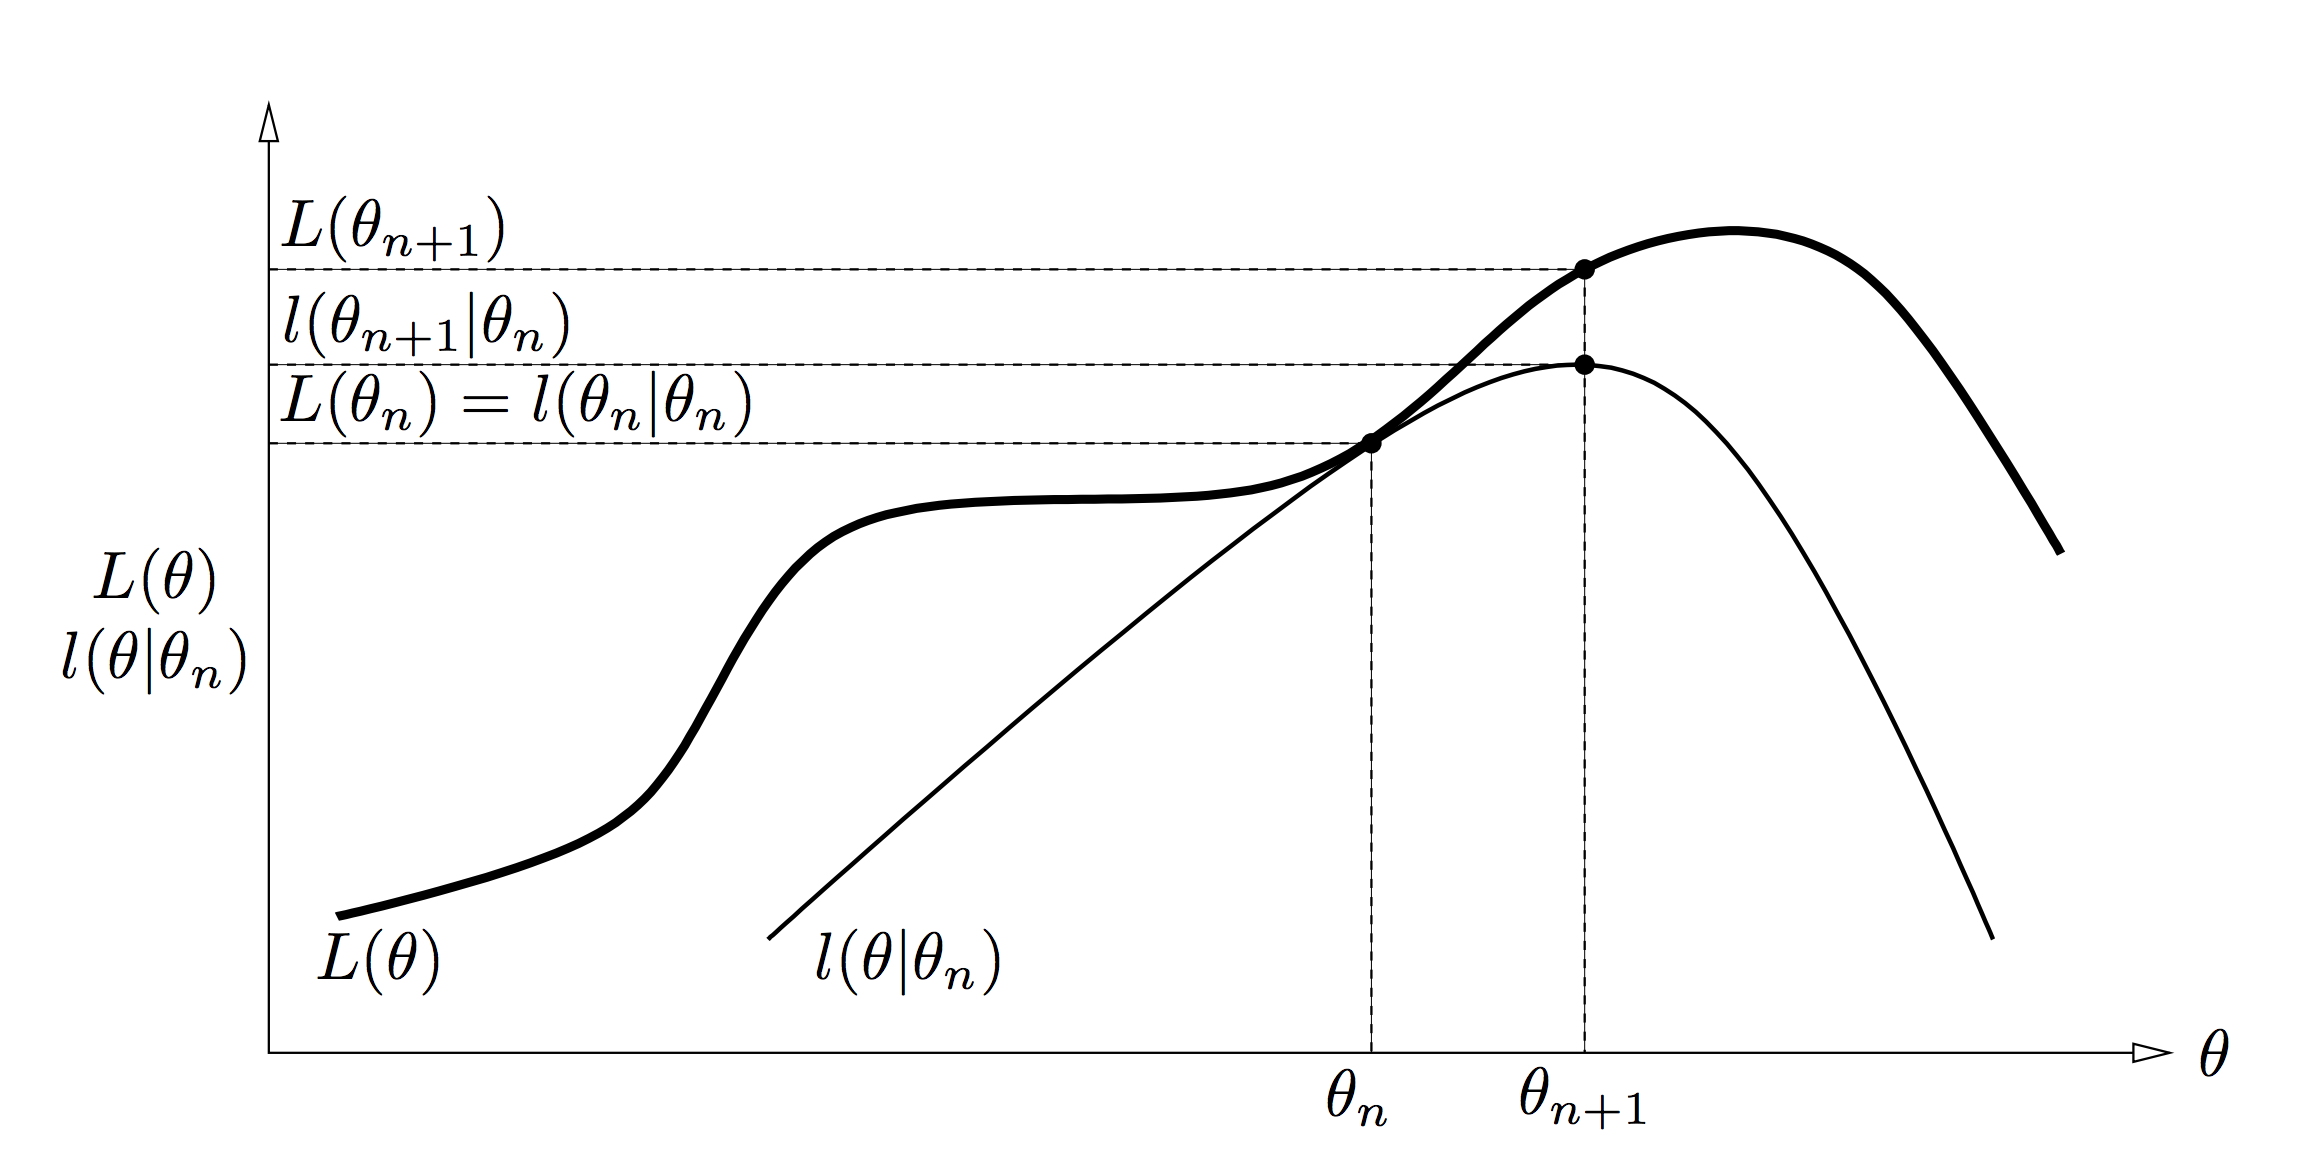
\includegraphics[width=1\textwidth,natwidth=610,natheight=642]{iter.png}
\caption{Graphical interpretation of a single iteration of the EM algorithm: The
function $l(\theta|\theta_n)$ is bounded above by the likelihood function $L(\theta)$. That is, the E-step constructs a function that lower bounds the likelihood function. The M-step finds $\theta_{n+1}$ that maximizes the function $l(\theta|\theta_n)$. Since $L(\theta) \geq l(\theta|\theta_n)$, increasing $l(\theta|\theta_n)$ ensures that the value of the likelihood function $L(\theta)$ is increased at each iteration.}
\label{fig:em}
\end{figure}%%%%%%%%%%%

so for $\theta=\theta_n$ the functions $l(\theta|\theta_n)$ and $L(\theta)$ are equal.

In order to achieve the greatest possible increase in the value of $L(\theta)$, the EM algorithm calls for selecting $\theta$ such that $l(\theta|\theta_n)$ is maximized. We denote this update as $\theta_{n+1}$. This whole process is illustrated in Fig.~\ref{fig:em}.


Formally we have,
\begin{align*}
\theta_{n+1} = &\arg\max _\theta \{ l(\theta|\theta_n)\} \\
 = & \arg\max\left\{L(\theta_n) +  \sum_z P(z|y,\theta_n)\cdot \log \left(\frac{P(y|z,\theta)P(z|\theta)}{P(z|y,\theta_n)P(y|\theta_n)} \right)\right\}\\
 & \text {now dropping terms which are constant with respect to $\theta$}\\
 = & \arg\max_\theta \left\{ \sum_z P(z|y,\theta_n) \log P(y|z,\theta) P(z|\theta)  \right\}\\
 = & \arg\max_\theta \left\{ \sum_z P(z|y,\theta_n) \log \frac{P(y,z,\theta)}{P(z,\theta)} \frac{P(z,\theta)}{P(\theta)} \right\}\\
  = & \arg\max_\theta \left\{ \sum_z P(z|y,\theta_n) \log P(y,z|\theta) \right\}\\
\label{eqn:em}  = & \arg\max_\theta \left\{ E_{z|y,\theta_n} \{\log P(y,z|\theta)\} \right\}\\
\end{align*}
The EM algorithm thus consists of iterating the:
\begin{enumerate}
\item E-step: Determine the conditional expectation $E_{z|y,\theta_n} \{\log P(y,z|\theta)\}$;
\item M-step: Maximize this expression with respect to $\theta$.
\end{enumerate}

We have simply traded the maximization of $L(\theta)$ for the maximization of $l(\theta|\theta_n)$. Given knowledge of the hidden variables, $l(\theta|\theta_n)$ takes into account the unobserved or the missing data $z$, so that the maximization of $l(\theta|\theta_n)$ is simplified. 

\begin{thebibliography}{9}

\bibitem{nature} Chuong B Do,  Serafim Batzoglou, \emph{What is the expectation maximization algorithm}, Nature Biotechnology 26, 897-899, dpi:10.1038/nbt14052008, \url{http://www.nature.com/nbt/journal/v26/n8/full/nbt1406.html}.

\bibitem{slides} UCSB Bioinformatics course slides, \url{http://www.cs.ucsb.edu/~ambuj/Courses/bioinformatics/EM.pdf}

\bibitem{sb} Sean Borman, \emph{The Expectation Maximization Algorithm: a Short Tutorial}, \url{http://www.seanborman.com/publications/EM_algorithm.pdf}

\bibitem{em_mb} Moritz Blume, \emph{Expectation Maximization: A Gentle
Introduction},
\url{http://campar.in.tum.de/twiki/pub/Main/MoritzBlume/EMGaussianMix.pdf}

\bibitem{lagrange} Dan Klein, \emph{Lagrange multiplier without permanent
scarring}, University of California at Berkeley, Computer Science Division.

\bibitem{demystified} Yihua Chen \& Maya R. Gupta, \emph{EM Demystified: An
Expectation-Maximization Tutorial}, Department of Electrical Engineering,
University of Washington, Seattle, WA, February 2010. \url{https://www.ee.washington.edu/techsite/papers/documents/UWEETR-2010-0002.pdf}

\end{thebibliography}


\end{document}
